\documentclass[10pt,twocolumn]{article}
\usepackage[utf8]{inputenc}
\usepackage[T1]{fontenc}
\usepackage[letterpaper,margin=0.75in,columnsep=0.25in]{geometry}
\usepackage{newtxtext,newtxmath}
\usepackage{microtype}
\usepackage[font=small,labelfont=bf,labelsep=period]{caption}
\renewcommand{\topfraction}{0.9}
\renewcommand{\dbltopfraction}{0.9}
\renewcommand{\textfraction}{0.1}
\renewcommand{\floatpagefraction}{0.8}
\renewcommand{\dblfloatpagefraction}{0.8}
\setcounter{topnumber}{3}
\setcounter{dbltopnumber}{3}
\usepackage{amsmath}
\usepackage{graphicx}
\graphicspath{{figures/}{./}}
\usepackage{booktabs}
\usepackage{tikz}
\usetikzlibrary{positioning,arrows.meta}
\usepackage[hidelinks]{hyperref}

\title{3D Reconstruction by Multi-View Photometric Stereo\\with a Custom-Built LED Dome}
\author{Justin Desrochers\\Polytechnique Montr\'eal}
\date{November 2026}

\begin{document}
\maketitle

\begin{abstract}
In this project I built a low-cost LED dome for multi-view photometric stereo, I designed it, 3D printed it, wired it and assembled it myself from scratch. The dome have 16 calibrated LEDs, an industrial camera and a motorized turntable, and everything is controlled by one microcontroller. A full scan, under every light and for every angle of the turntable, is launched with a single command from the computer. To know where the camera is, I glued the object on a checkerboard, and then all the images are fused in one textured mesh with a neural photometric stereo network and a neural signed distance surface. On a chess knight of 40~mm, the final model match the real dimensions to about 2\% and it agree with the input silhouettes with a median IoU of 0.971. The motivation is to reduce the domain gap between synthetic training data and real images, by capturing real objects instead of modelling them by hand.
\end{abstract}

\section{Introduction}
Making realistic 3D assets by hand in Maya, Blender or Houdini take a lot of time, and in the end the result is only the approximation of an artist, not the real object. A faster way is to capture the real object directly and transform it in a textured 3D model that we can use as synthetic data. But photos alone are not enough for that. In one photo, the shape of the object, its colour and the lighting are all mixed together, so the shadows and the highlights end up baked in the texture. To separate them, you need a controlled setup, with lights at known positions, a calibrated camera and a known rotation of the object between the views. This is why I went with a dome. Compared to a normal photo setup, every light is fixed at a known position and the room light is blocked, so each image is taken under a light that we control and that is calibrated. Then photometric stereo use the change of brightness between the lights to find the orientation of the surface at every pixel, which keep the small details that multi-view geometry alone usually smooth out. This paper present the system I built, a 3D-printed LED dome for multi-view photometric stereo. The long-term goal is to make the generation of synthetic data faster, and since it work for basically any object that fit in the dome, it is not really limited to one specific field.

\section{Related Work}
\paragraph{Photometric stereo.} Photometric stereo was introduced by Woodham~\cite{woodham1980}. He showed that a few images under different lights are enough to find the orientation of every point on a surface. The original method assume distant lights of equal power. In my case the LEDs are close to the object, so this is not true anymore, and the position, the power and the beam of each LED need to be modelled and calibrated~\cite{queau2018}. More recently, neural networks like SDM-UniPS~\cite{ikehata2023} estimate the normals and the albedo directly from the images, without requiring the light positions.

\paragraph{Multi-view reconstruction.} One photometric stereo view only describe the side of the object that the camera see. To have a complete model, you have to combine many views. Neural implicit methods like NeuS~\cite{wang2021} and NeuS2~\cite{wang2023} represent the surface as a signed distance function that is learned from the images. RNb-NeuS~\cite{brument2024} and after it RNb-NeuS2~\cite{bruneau2026} bring this idea to photometric stereo data, they use the normal and albedo maps of every view to optimize one single surface.

\paragraph{Evaluation.} To know how accurate a 3D scan is, you need a reference shape. Usually people use expensive laser scanners for this. The MobileBrick dataset~\cite{li2023} use LEGO models instead, because their exact 3D shape is known from the building instructions.

In this work I put these pieces together in one low-cost system. The dome, the electronics and the calibration are all made by me from scratch, and for the reconstruction I used existing neural methods.

\section{Background}
Photometric stereo~\cite{woodham1980} find the orientation of a surface from images taken by a camera that don't move, under different lights. The intensity of a pixel depend on the angle between the surface normal and the light direction, so by changing only the light, the shading encode the local orientation of the surface. For a matte (Lambertian) surface, the brightness of a pixel under the light $k$ is
\begin{equation}
I_k = \rho\,\max(\mathbf{n}\cdot\mathbf{l}_k, 0),
\end{equation}
where $\rho$ is the albedo, $\mathbf{n}$ the surface normal and $\mathbf{l}_k$ the direction of the light. If we write $\mathbf{g} = \rho\,\mathbf{n}$ and we stack the $m$ lights, we get the linear system $\mathbf{I} = L\,\mathbf{g}$, with three unknowns for each pixel. With $m \geq 3$ lights, it can be solved with least squares,
\begin{equation}
\hat{\mathbf{g}} = (L^\top L)^{-1} L^\top \mathbf{I}, \qquad \hat{\rho} = \|\hat{\mathbf{g}}\|, \qquad \hat{\mathbf{n}} = \hat{\mathbf{g}} / \|\hat{\mathbf{g}}\|.
\end{equation}
Since each pixel is solved independently, photometric stereo recover high-frequency details such as small bumps and engravings. However, a single view only constrain the gradient of the visible surface, not the full shape of the object. Integrating the normal field of one view tend to lose the global depth, so a complete model require combining many views around the object.

\begin{figure*}[!t]
\centering
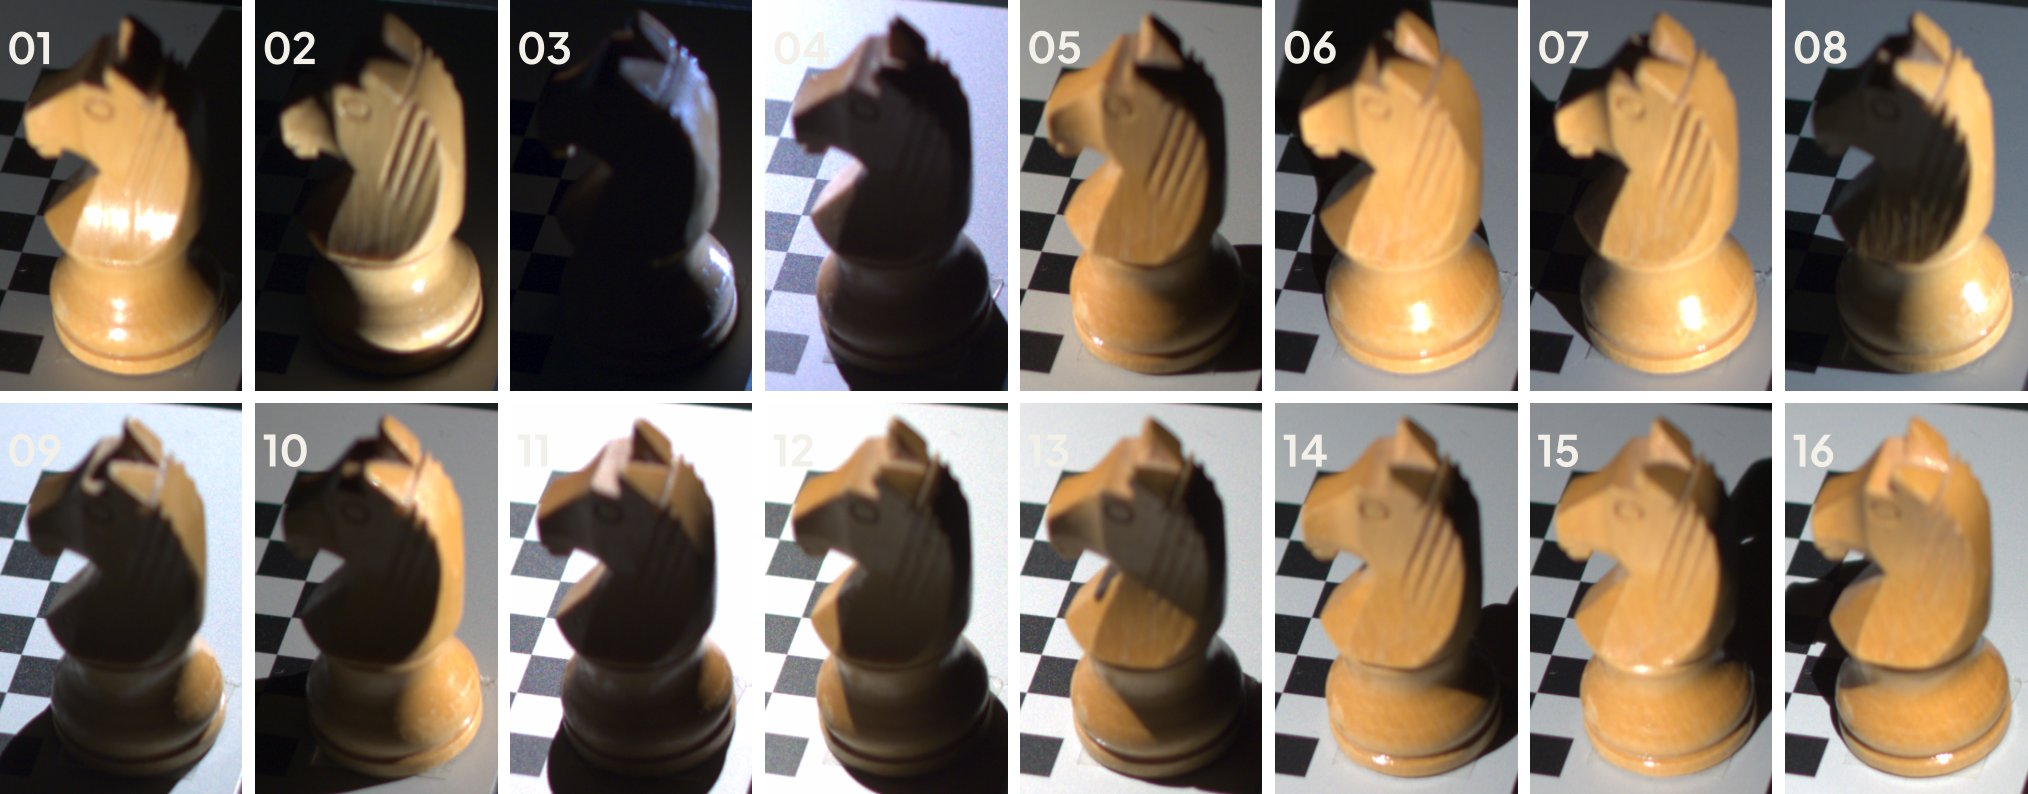
\includegraphics[width=\textwidth]{sixteen_lights.jpg}
\caption{One view of the knight under each of the 16 LEDs. The camera and the object don't move, only the light is changing.}
\label{fig:lights}
\end{figure*}

\section{Hardware}
The system have four parts: a dome that hold the lights, a camera, a turntable and a controller that synchronize everything.

\paragraph{Dome.} The dome is a 2V geodesic shell with a radius of 300~mm, made of 40 triangle panels printed in black ASA. I chose ASA because it is stiff and resist to heat, so the LEDs stay at the same position once the dome is assembled. The shell is closed and black, so it also block the room light, which mean that the only light that reach the object come from the dome.

\paragraph{LEDs.} There is sixteen Luxeon SW-01 white LEDs mounted at three heights (5, 10 and 1 LEDs). Photometric stereo need at least three lights to solve the normal of a surface. With sixteen, the system is over-determined, so the least squares average the noise of the image, and a point can still be solved even if some LEDs are hidden by the object or make a specular highlight. Putting the LEDs at different heights also change the elevation of the light, and this make the system better conditioned. Each LED is driven by an LM317 constant-current source at around 320~mA, so its brightness stay stable from one capture to the other.

\paragraph{Camera.} A LUCID Triton TRI050S-CC 5~MP colour industrial camera with a Fujinon HF25XA-5M 25~mm lens look at the object through an oblique port at $52.6^\circ$ of elevation. One pixel cover about 0.059~mm on the object, so the field of view is around $14 \times 12$~cm, which limit the size of the object to about 12~cm. The controller trigger the camera, and the camera record raw Bayer images with a fixed exposure. Raw images are important here, because photometric stereo suppose that the value of a pixel is proportional to the light it receive, and the gamma curve and the automatic exposure of a consumer camera break this assumption.

\paragraph{Turntable.} The object sit on a turntable of 160~mm driven by a NEMA~17 stepper motor and a TMC2209 driver, with 3{,}200 microsteps per turn. Between each view the object turn of $10^\circ$, so we get 36 views per turn without touching it by hand, and the rotation is always the same.

\paragraph{Controller.} An Arduino Mega run all the capture. At each position, it turn on one LED, take one photo, do this again for the 16 LEDs, and then turn the object of $10^\circ$. The whole sequence run without any manual step, you just start it with one command on the computer. On the front there is a panel with an OLED screen, a status light, three buttons (red, yellow and green) and a power switch, to see the state of the dome and control it. All the electronics is mounted on the dome, so it can be unplugged and lifted from its base to place or turn the object. The wiring diagrams, the bill of materials and the assembly guide are in the project repository.

\begin{figure*}[!t]
\centering
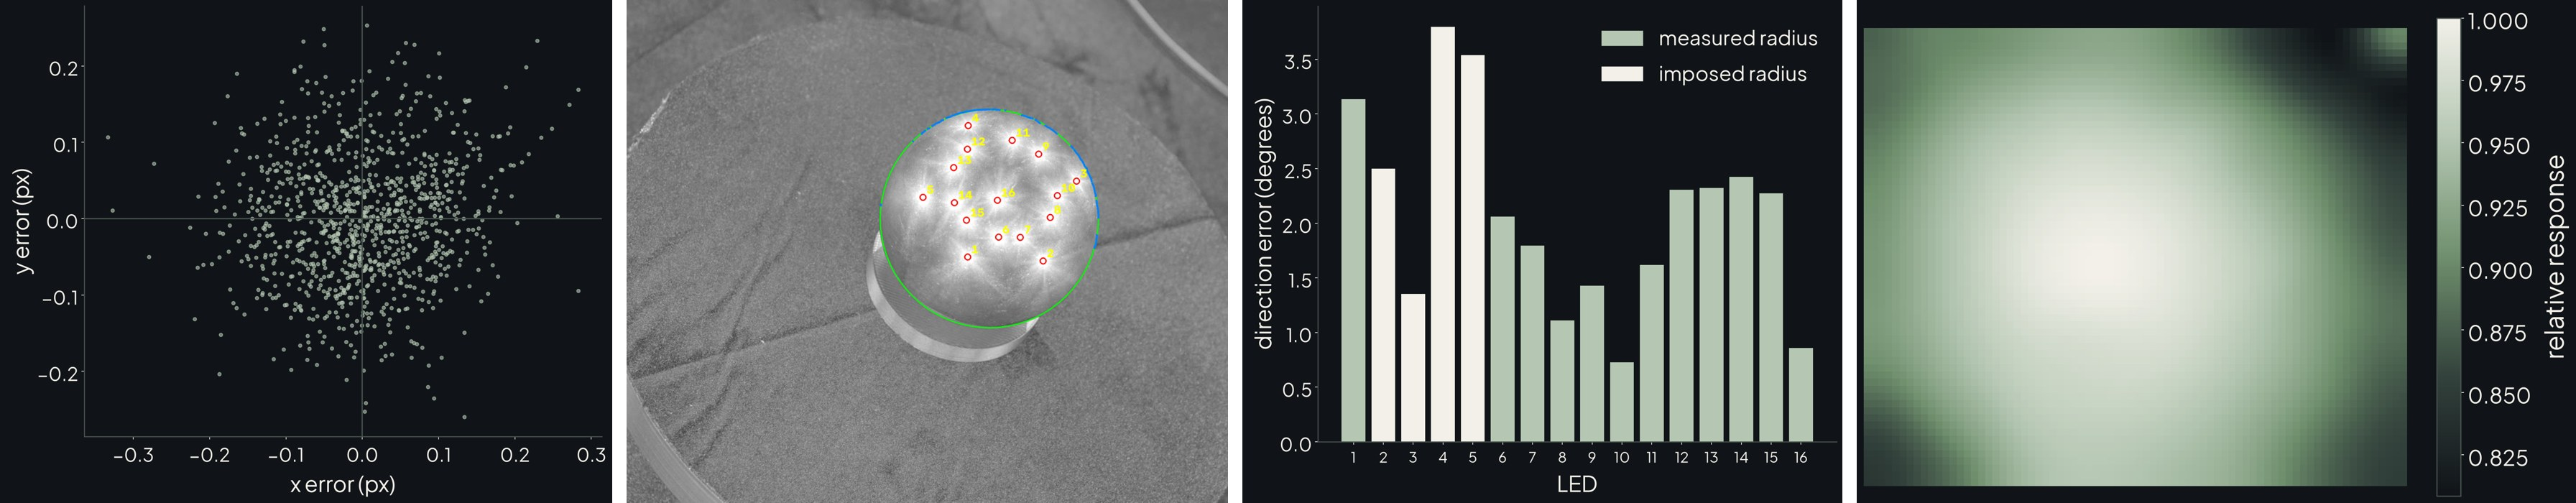
\includegraphics[width=\textwidth]{calibration.jpg}
\caption{Calibration results, from left to right. (a) Reprojection error of the checkerboard corners (median 0.10~px). (b) Highlights of the 16 LEDs detected on the mirror ball. (c) Direction error of each LED compared to the CAD model. (d) Relative light response across the image, measured on the white plate.}
\label{fig:calib}
\end{figure*}

\section{Calibration}
The basic photometric stereo model assume distant lights of equal power. In my dome the LEDs are only at 300~mm from the object, so the direction of the light change across the object, the intensity drop with the squared distance, and each LED emit less light away from its optical axis. A more complete model of the image is
\begin{equation}
I_k(\mathbf{x}) = E_k\,\rho(\mathbf{x})\,\frac{\max(\mathbf{n}\cdot\mathbf{l}_k(\mathbf{x}),0)}{\|\mathbf{s}_k-\mathbf{x}\|^2}\,D_k(\mathbf{x}),
\end{equation}
where $E_k$ is the power of the LED $k$, $\mathbf{s}_k$ its position and $D_k$ its beam profile. Also, I assembled the dome by hand, so the real values are not exactly the ones of the CAD model. So I measured each of these parameters with a calibration object made for it.

\paragraph{Camera.} With a checkerboard in 12 poses, I got the intrinsic matrix $K$ and the lens distortion with the method of Zhang~\cite{zhang2000}. The median reprojection error is 0.10~px (RMS 0.123~px), and the maximum distortion of the lens is 13.4~px, which confirm that it must be corrected.

\paragraph{LED positions.} I put a mirror ball at the centre of the turntable, and each LED make a small highlight on it. The position of this highlight on the ball give the direction of the LED. Compared to the CAD model, the median error on the direction is $2.2^\circ$ (maximum $3.8^\circ$). The distances are less precise, with a median error of 17~mm (maximum 79~mm).

\paragraph{LED power and vignetting.} All the LEDs receive the same current, but they don't give the same amount of light. I took photos of a flat white plate under each LED, which give the relative power of each one, going from 0.79 to 1.34 times the mean, and also how the light change across the image. I also took the same plate with two exposure times (10 and 35~ms) to check if the camera response is linear, and I measured a ratio of 3.51 when 3.50 was expected.

\begin{figure*}[!t]
\centering
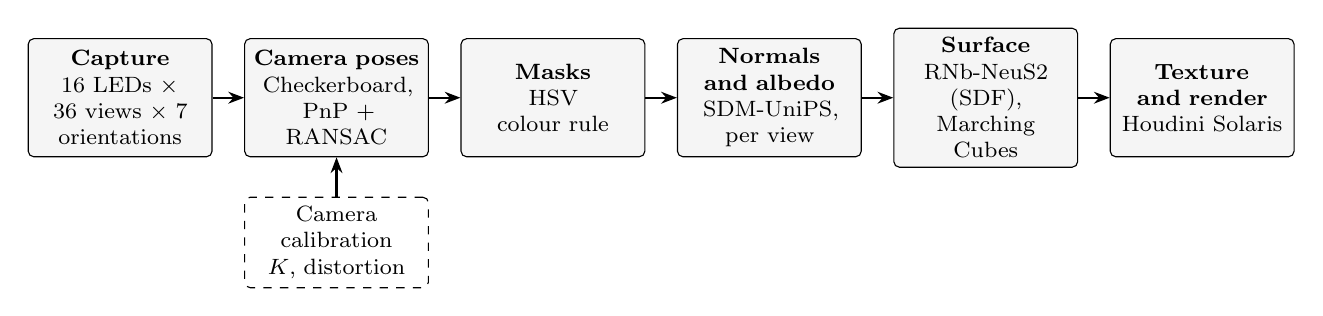
\begin{tikzpicture}[
  box/.style={draw, rounded corners=2pt, align=center, text width=2.1cm, minimum height=1.5cm, font=\footnotesize, fill=gray!8},
  side/.style={draw, dashed, rounded corners=2pt, align=center, text width=2.1cm, minimum height=0.9cm, font=\footnotesize},
  arr/.style={-{Stealth[length=2mm]}, thick},
  node distance=0.4cm]
\node[box] (cap) {\textbf{Capture}\\16 LEDs $\times$ 36 views $\times$ 7 orientations};
\node[box, right=of cap] (pose) {\textbf{Camera poses}\\Checkerboard,\\PnP + RANSAC};
\node[box, right=of pose] (mask) {\textbf{Masks}\\HSV colour rule};
\node[box, right=of mask] (norm) {\textbf{Normals and albedo}\\SDM-UniPS, per view};
\node[box, right=of norm] (surf) {\textbf{Surface}\\RNb-NeuS2 (SDF),\\Marching Cubes};
\node[box, right=of surf] (tex) {\textbf{Texture and render}\\Houdini Solaris};
\node[side, below=0.5cm of pose] (cal) {Camera calibration\\$K$, distortion};
\draw[arr] (cap) -- (pose);
\draw[arr] (pose) -- (mask);
\draw[arr] (mask) -- (norm);
\draw[arr] (norm) -- (surf);
\draw[arr] (surf) -- (tex);
\draw[arr] (cal) -- (pose);
\end{tikzpicture}
\caption{Overview of the reconstruction pipeline. The poses, masks, normals and albedo of all the views are used together to optimize one single surface.}
\label{fig:pipeline}
\end{figure*}

\section{Reconstruction Pipeline}
Figure~\ref{fig:pipeline} show the whole pipeline, from the raw images to the textured model. I will go through it step by step.

\paragraph{Test object and capture.} For the test object I used a chess knight, because it is small (40~mm high) and it have a lot of fine details. I captured the knight in 7 orientations, five for the top and the sides and two for the bottom. Each orientation give 36 views of the turntable under 16 LEDs, so in total it's $7 \times 36 \times 16 = 4{,}032$ raw images (around 50~GB). One orientation of 576 images take about one minute, so almost ten images per second, and the full capture take around seven minutes plus the time to turn the object by hand. From all this, I kept 168 views for the reconstruction.

\paragraph{Camera poses.} I glued the knight on the calibration checkerboard, so the board is also visible in every image. Then the pose of the camera for each view is measured directly, by minimizing the reprojection error of the corners of the board,
\begin{equation}
\min_{R,\mathbf{t}} \sum_i \left\| \mathbf{u}_i - \pi\!\left(K, \mathbf{d}, R\mathbf{X}_i + \mathbf{t}\right) \right\|^2,
\end{equation}
which I solved with PnP and RANSAC~\cite{fischler1981}. The pose was found in 33 to 36 of the 36 views of each orientation, with consistency checks between 0.2 and 0.5~mm.

\paragraph{Masks.} The board is black and white and the knight have colour, so a simple rule in the HSV space can separate them. A pixel is part of the object when its saturation $S > 70$ and its value $V > 35$. I expected the SAM segmentation model~\cite{kirillov2023} to perform better, but this simple rule gave cleaner contours. The limitation is that it would fail on an object without colour (Fig.~\ref{fig:masks}).

\begin{figure}[t]
\centering
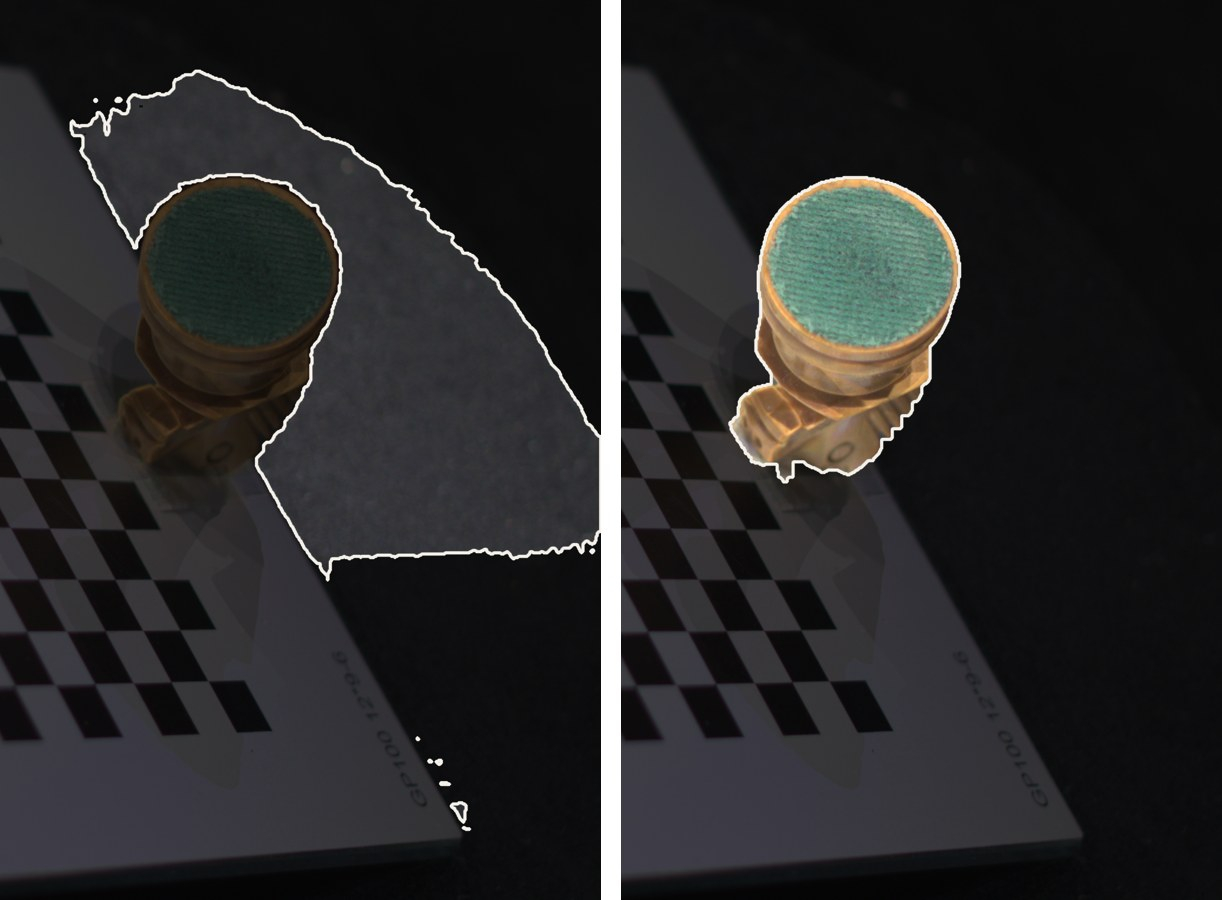
\includegraphics[width=\linewidth]{masks.jpg}
\caption{Masks of the object for the same view, with the knight glued on the checkerboard. Left, SAM take a part of the board. Right, the colour rule follow the contour of the knight.}
\label{fig:masks}
\end{figure}

\paragraph{Normals and albedo.} The normals and the albedo of the surface are estimated in each view with SDM-UniPS~\cite{ikehata2023}, a neural network for universal photometric stereo. At first I used the normals computed from the calibrated light model, but for the same point of the surface, they were different by $12^\circ$ to $17^\circ$ from one view to the other, so I replaced them by the network. Figure~\ref{fig:maps} show what the network give for three orientations.

\begin{figure*}[!t]
\centering
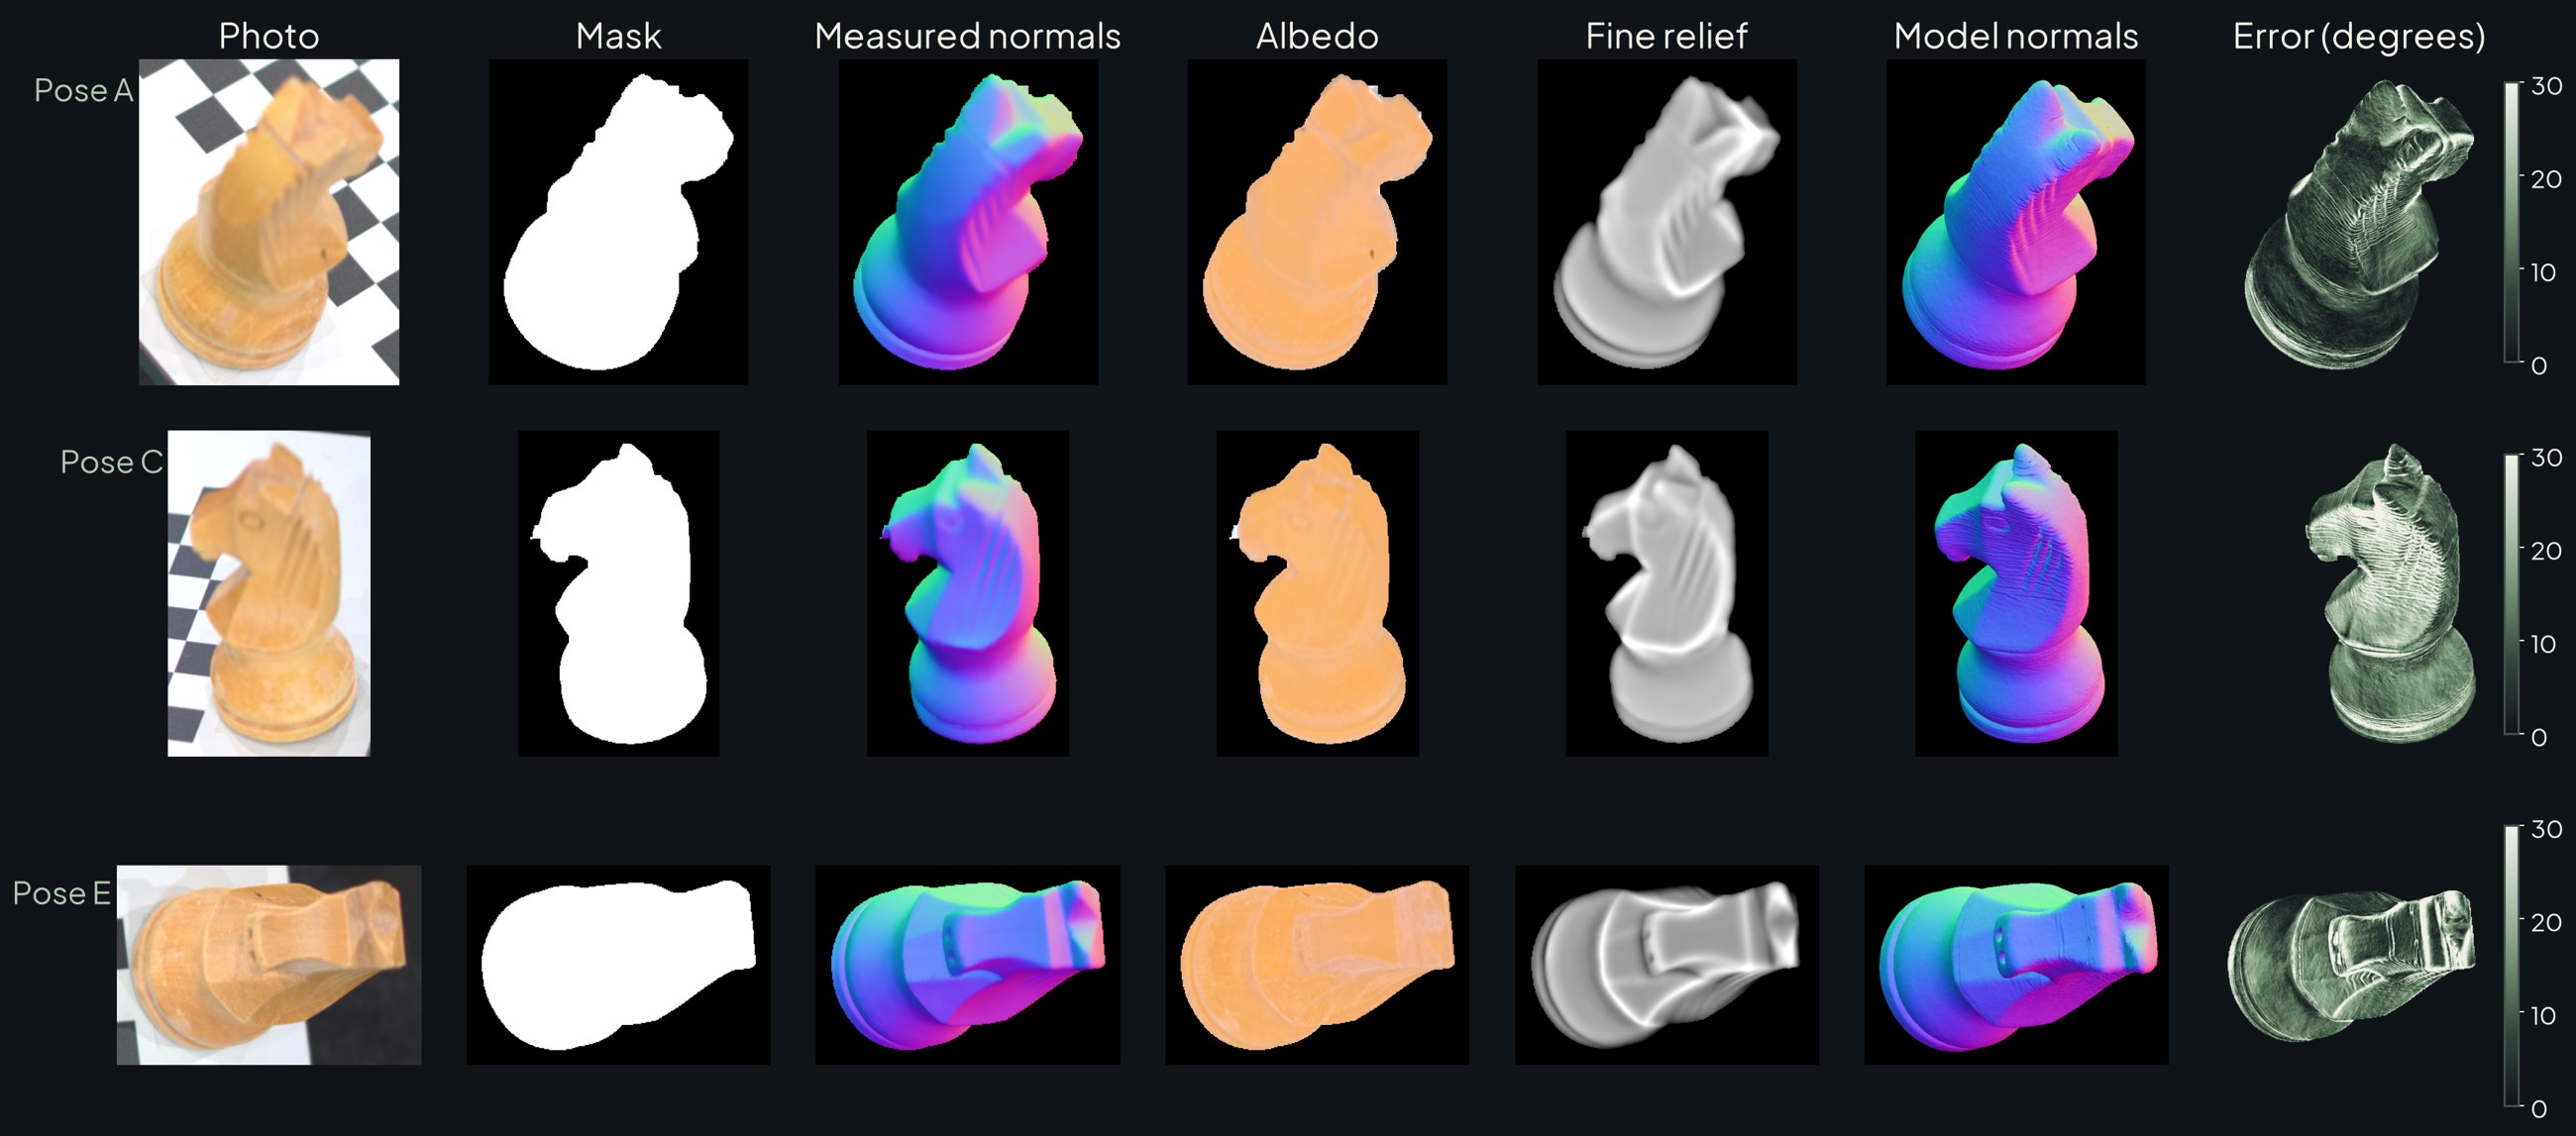
\includegraphics[width=\textwidth]{maps_results.jpg}
\caption{Results for three orientations of the knight. From left to right, input photo, mask, normals measured by SDM-UniPS, albedo, fine relief, normals of the reconstructed surface, and angular error between the measured normals and the normals of the reconstructed surface.}
\label{fig:maps}
\end{figure*}

\paragraph{Surface reconstruction.} All the views are fused in one surface with RNb-NeuS2~\cite{bruneau2026}. The surface is the zero level of a signed distance function $f$,
\begin{equation}
S = \{\mathbf{x} : f(\mathbf{x}) = 0\}, \qquad \mathbf{n} = \frac{\nabla f}{\|\nabla f\|}.
\end{equation}
Each pair of normal and albedo is converted in brightness values $\mathbf{v}_k$ under some virtual lights, and the method minimize
\begin{equation}
\min_{f,\rho} \sum_k \left\| \tilde{\mathbf{v}}_k(f,\rho) - \mathbf{v}_k \right\|_p^p + \lambda\,\mathcal{L}_{\mathrm{eik}} + \mathcal{L}_{\mathrm{mask}},
\end{equation}
where $\tilde{\mathbf{v}}_k$ is rendered from the current surface. The eikonal term $\mathcal{L}_{\mathrm{eik}} = \mathbb{E}\big[(\|\nabla f\|-1)^2\big]$ keep $f$ a real distance, and the mask term keep the shape coherent with the contours of the object. The main advantage of this formulation is that every view constrain the same surface, so no separate partial models need to be merged afterwards. Because of the memory of the GPU I had, the optimization run at half resolution for 20{,}000 iterations, and not all the captured views are used. Then Marching Cubes extract a mesh of 615{,}974 triangles.

\paragraph{Texture and rendering.} I imported the mesh in Houdini and applied the albedo from the pipeline as a texture. The final scene is built and rendered in Houdini Solaris, so the model can be relit under any lighting. The roughness of the wood is not measured, I set it by hand in the material, with a bump map for the small details of the surface.

\subsection{Design decisions}
My first reconstructions were not recognizable as the knight. I tried many simpler methods before arriving to this pipeline, and two failures really decided the final design. First, when I integrated the normals of each view with Poisson reconstruction, the object came out flat, with a depth of 6~mm instead of 25~mm, because the vertical walls of the knight were lost. After that, the partial models could not be fitted together. Second, when I aligned these partial models with ICP, it often converged to a mirrored solution, since the knight is almost symmetric. This is why the poses now come from the checkerboard instead of being estimated from the object. Table~\ref{tab:decisions} resume all the methods I tested.
\begin{table*}[!t]
\centering
\small
\begin{tabular}{@{}llll@{}}
\toprule
Step & Tried & Problem & Kept \\
\midrule
Shape & Poisson, visual hull, TSDF & Flat, artifacts & RNb-NeuS2 \\
Alignment & ICP on 3D models & Mirror solutions & PnP + RANSAC \\
Masks & SAM & Visible errors & Colour rule \\
Normals & Calibrated light model & $12$--$17^\circ$ between views & SDM-UniPS \\
\bottomrule
\end{tabular}
\caption{Methods I tested and the one I kept at each step.}
\label{tab:decisions}
\end{table*}

\section{Results}
The final model is a complete textured mesh of the knight, and it can be relit under any lighting (Fig.~\ref{fig:knight}).

\begin{figure*}[!t]
\centering
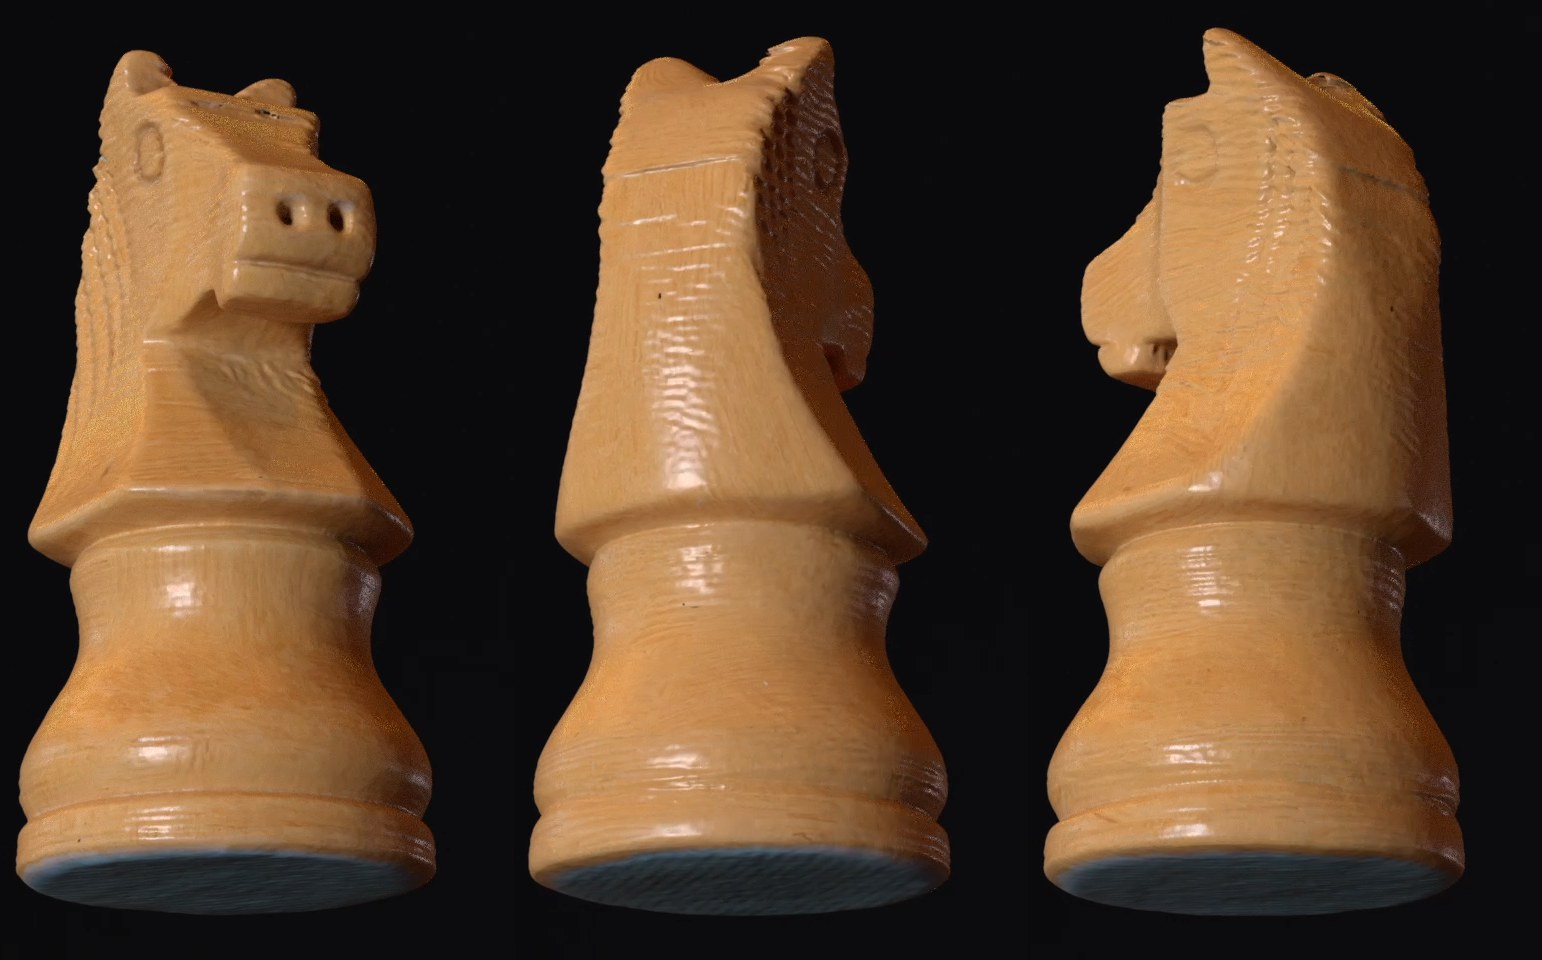
\includegraphics[width=0.85\textwidth]{knight_render.jpg}
\caption{The reconstructed knight seen from three sides, rendered in Houdini Solaris.}
\label{fig:knight}
\end{figure*}
 I compared its overall dimensions with caliper measurements of the real object (Table~\ref{tab:size}). The height and the width of the base are both within about 2\% of the real values, and the model is slightly larger in both directions.

\begin{table}[!t]
\centering
\small
\begin{tabular}{@{}lccc@{}}
\toprule
 & Model & Real & Difference \\
\midrule
Height & 40.87~mm & 40.00~mm & +0.87~mm (2.2\%) \\
Base width & 19.17~mm & 18.85~mm & +0.32~mm (1.7\%) \\
\bottomrule
\end{tabular}
\caption{Overall size of the reconstructed knight.}
\label{tab:size}
\end{table}

I also did two other checks to see if the model agree with its input data. Its silhouettes overlap the masks of the object with a median IoU of 0.971, and its surface normals are different from the normals measured by photometric stereo by a median of $11.0^\circ$ (Fig.~\ref{fig:maps}, last column). These numbers show that the model is coherent with its own images. But they don't measure the absolute accuracy, because I don't have a 3D ground truth of the knight.

\section{Limitations and Future Work}
The biggest limitation is that I don't have a 3D ground truth. The overall size of the knight is correct to about 2\%, but the accuracy of the surface itself and of the fine details is not measured yet. The model is also a little bigger than the real object in the two directions I measured, so there is probably a small systematic scale bias. Other limits come from my choices in the pipeline. The colour mask only work on objects with colour, the field of view limit the objects to about 12~cm, and the normals from the calibrated light model were not precise enough to be used in the final reconstruction. The reconstruction also run at half resolution on only part of the views because of the GPU memory, so some of the detail captured by the camera is lost. Finally, only the shape and the albedo are measured. The roughness is set by hand, and transparent or very shiny materials are not supported.

To measure the accuracy of the surface, the next step is a validation with LEGO models, like in the MobileBrick dataset~\cite{li2023}. LEGO bricks are made with a tolerance of about 0.01~mm, and a built model is different from its 3D file by about 0.2~mm on average, so we know the exact shape without needing an expensive scanner. My plan is to build a coloured LEGO model from a 3D file, capture it with the same pipeline, and align it with its digital model to compute the Chamfer distance and the F1 score.

There is also some improvements that would make the system closer to a real synthetic data tool. With a GPU with more memory, the reconstruction could run at full resolution with all the views. Capturing the roughness and the transparency of the surface, and not only the albedo, would give more realistic materials. The next objects should also be organic shapes that are hard to model by hand, because it's there that capturing a real object is the most useful. And finally, the scanned models can go in a node-based pipeline in Houdini that change automatically the lighting, the camera, the background and the materials, to produce labelled images for training AI models.

\section{Conclusion}
In this project I built a 3D-printed LED dome for multi-view photometric stereo, and I went through all the steps, from the hardware and the calibration to a complete textured 3D model. The main thing I learned is that measuring with a rigid reference work better than estimating from the object itself, and that's why the camera poses come from a checkerboard glued under the object. The first scans were not recognizable, while the final pipeline now produce a realistic model with measured shape, normals and texture. The reconstructed knight match the real object to about 2\% in size and agree well with its own images. For me this is a first step towards a tool that make the creation of realistic synthetic data from real objects faster. All the design files, the code and the assembly instructions are available on GitHub: \url{https://github.com/Juju-dotcom/dome-ps16}.

\section*{Acknowledgments}
I want to thank L\'eane Tremblay, student in electrical engineering, for her help with the electronics of the dome.

\begin{thebibliography}{9}
\bibitem{woodham1980} R.~J. Woodham, ``Photometric method for determining surface orientation from multiple images,'' \emph{Optical Engineering}, vol.~19, no.~1, pp.~139--144, 1980.
\bibitem{zhang2000} Z.~Zhang, ``A flexible new technique for camera calibration,'' \emph{IEEE Trans. Pattern Analysis and Machine Intelligence}, vol.~22, no.~11, pp.~1330--1334, 2000.
\bibitem{fischler1981} M.~A. Fischler and R.~C. Bolles, ``Random sample consensus,'' \emph{Communications of the ACM}, vol.~24, no.~6, pp.~381--395, 1981.
\bibitem{kirillov2023} A.~Kirillov \emph{et al.}, ``Segment anything,'' in \emph{Proc. ICCV}, 2023.
\bibitem{ikehata2023} S.~Ikehata, ``Scalable, detailed and mask-free universal photometric stereo,'' in \emph{Proc. CVPR}, 2023.
\bibitem{li2023} K.~Li \emph{et al.}, ``MobileBrick: Building LEGO for 3D reconstruction on mobile devices,'' in \emph{Proc. CVPR}, 2023.
\bibitem{queau2018} Y.~Qu\'eau, B.~Durix, T.~Wu, D.~Cremers, F.~Lauze and J.-D. Durou, ``LED-based photometric stereo: Modeling, calibration and numerical solution,'' \emph{Journal of Mathematical Imaging and Vision}, vol.~60, pp.~313--340, 2018.
\bibitem{wang2021} P.~Wang \emph{et al.}, ``NeuS: Learning neural implicit surfaces by volume rendering for multi-view reconstruction,'' in \emph{Proc. NeurIPS}, 2021.
\bibitem{wang2023} Y.~Wang \emph{et al.}, ``NeuS2: Fast learning of neural implicit surfaces for multi-view reconstruction,'' in \emph{Proc. ICCV}, 2023.
\bibitem{brument2024} B.~Brument, R.~Bruneau, Y.~Qu\'eau, J.~M\'elou, F.~Lauze, J.-D. Durou and L.~Calvet, ``RNb-NeuS: Reflectance and normal-based multi-view 3D reconstruction,'' in \emph{Proc. CVPR}, 2024.
\bibitem{bruneau2026} Bruneau \emph{et al.}, RNb-NeuS2, 2026. % TODO: full reference
\end{thebibliography}

\end{document}
